\documentclass[tikz]{standalone}
\usepackage{tikz}
\usepackage{amsfonts}
\usepackage{amssymb}
\begin{document}

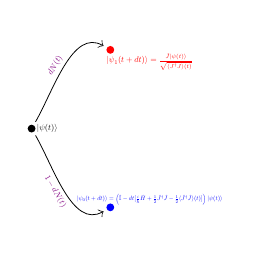
\begin{tikzpicture}
\coordinate (A) at (0,0);
\coordinate (B) at (1,1);
\coordinate (C) at (1,-1);
\node[fill=black,circle,scale=0.3] at (A) {};
\node[fill=red,circle,scale=0.3] at (B) {};
\node[fill=blue,circle,scale=0.3] at (C) {};
\draw[->,line width=0.1 mm, shorten <=0.1cm, shorten >= 0.1cm] (A) to[out=60,in=150] (B);
\draw[->,line width=0.1 mm,shorten <=0.1cm, shorten >= 0.1cm] (A) to[out=-60, in=-150] (C);
\node[scale=0.3,black] at (0.2,0) {$|\psi(t)\rangle$};
\node[scale=0.3,red] at (1.5,0.85) {$|\psi_{1}(t+dt)\rangle=\frac{\hat{J}|\psi(t)\rangle}{\sqrt{\langle\hat{J}^{\dagger}\hat{J}\rangle(t)}}$};
\node[scale=0.22,blue] at (1.5,-0.9) {$|\psi_{0}(t+dt)\rangle=\left(\hat{\mathbb{I}}-dt[\frac{i}{\hbar}\hat{H}+\frac{1}{2}\hat{J}^{\dagger}\hat{J}-\frac{1}{2}\langle\hat{J}^{\dagger}\hat{J}\rangle(t)]\right)|\psi(t)\rangle$};
\node[scale=0.3,blue!100!black!50!red!100!,rotate=-60] at (0.3,-0.8) {$1-dN(t)$};
\node[scale=0.3,blue!100!black!50!red!100!,rotate=60] at (0.3,0.8) {$dN(t)$};


\end{tikzpicture}

\end{document}